\documentclass{article}   	% use "amsart" instead of "article" for AMSLaTeX format
          		% ... or a4paper or a5paper or ... 
%\geometry{landscape}                		% Activate for rotated page geometry
%\usepackage[parfill]{parskip}    		% Activate to begin paragraphs with an empty line rather than an indent
\usepackage{graphicx}				% Use pdf, png, jpg, or eps§ with pdflatex; use eps in DVI mode
								% TeX will automatically convert eps --> pdf in pdflatex		
\usepackage{amssymb}
\usepackage{xcolor}
%SetFonts

%SetFonts

\usepackage{booktabs}

\title{Brief Article}
\author{The Author}
%\date{}							% Activate to display a given date or no date

\begin{document}
%\maketitle
%\section{}
%\subsection{}

\section{Introduction}

In this section I will provide a refresher on the work I was doing in August and September in Canberra.

\subsection{Generalized Divide the Dollar Game (GDD)}
The game is very straightforward. Each round $k>2$ players simultaneously announce how much of a dollar they are willing to accept. This announcement is referred to as a \textcolor{red}{\textit{bid}}.  If the bid total is $\le\$1$ then the players get their bid as a payoff. But, if the bid total exceeds $\$1$ the players get nothing.  A set of bids is considered \textcolor{blue}{\textit{coordinated}} if the bid total is $\le \$1$. The optimal solution would be a bid total of $\$1$ and a set of ``fair'' bids. 

A set of fair bids are roughly equal so no player is exploited. For example, suppose for simplicity there are only 2 players and the bids are $\{0.49, 0.51\}$. This has a bid total of $\$1$ and neither player is exploited. Now consider bids of $\{0.02, 0.98\}$. Here, too the bid total is $\$1$ but clearly the first player is exploited because his return is far less than that of the second player. You want a high bid total \textit{and} a fair set of bids.
See Figure \ref{fig1}.

\begin{figure}[htb]
\centerline{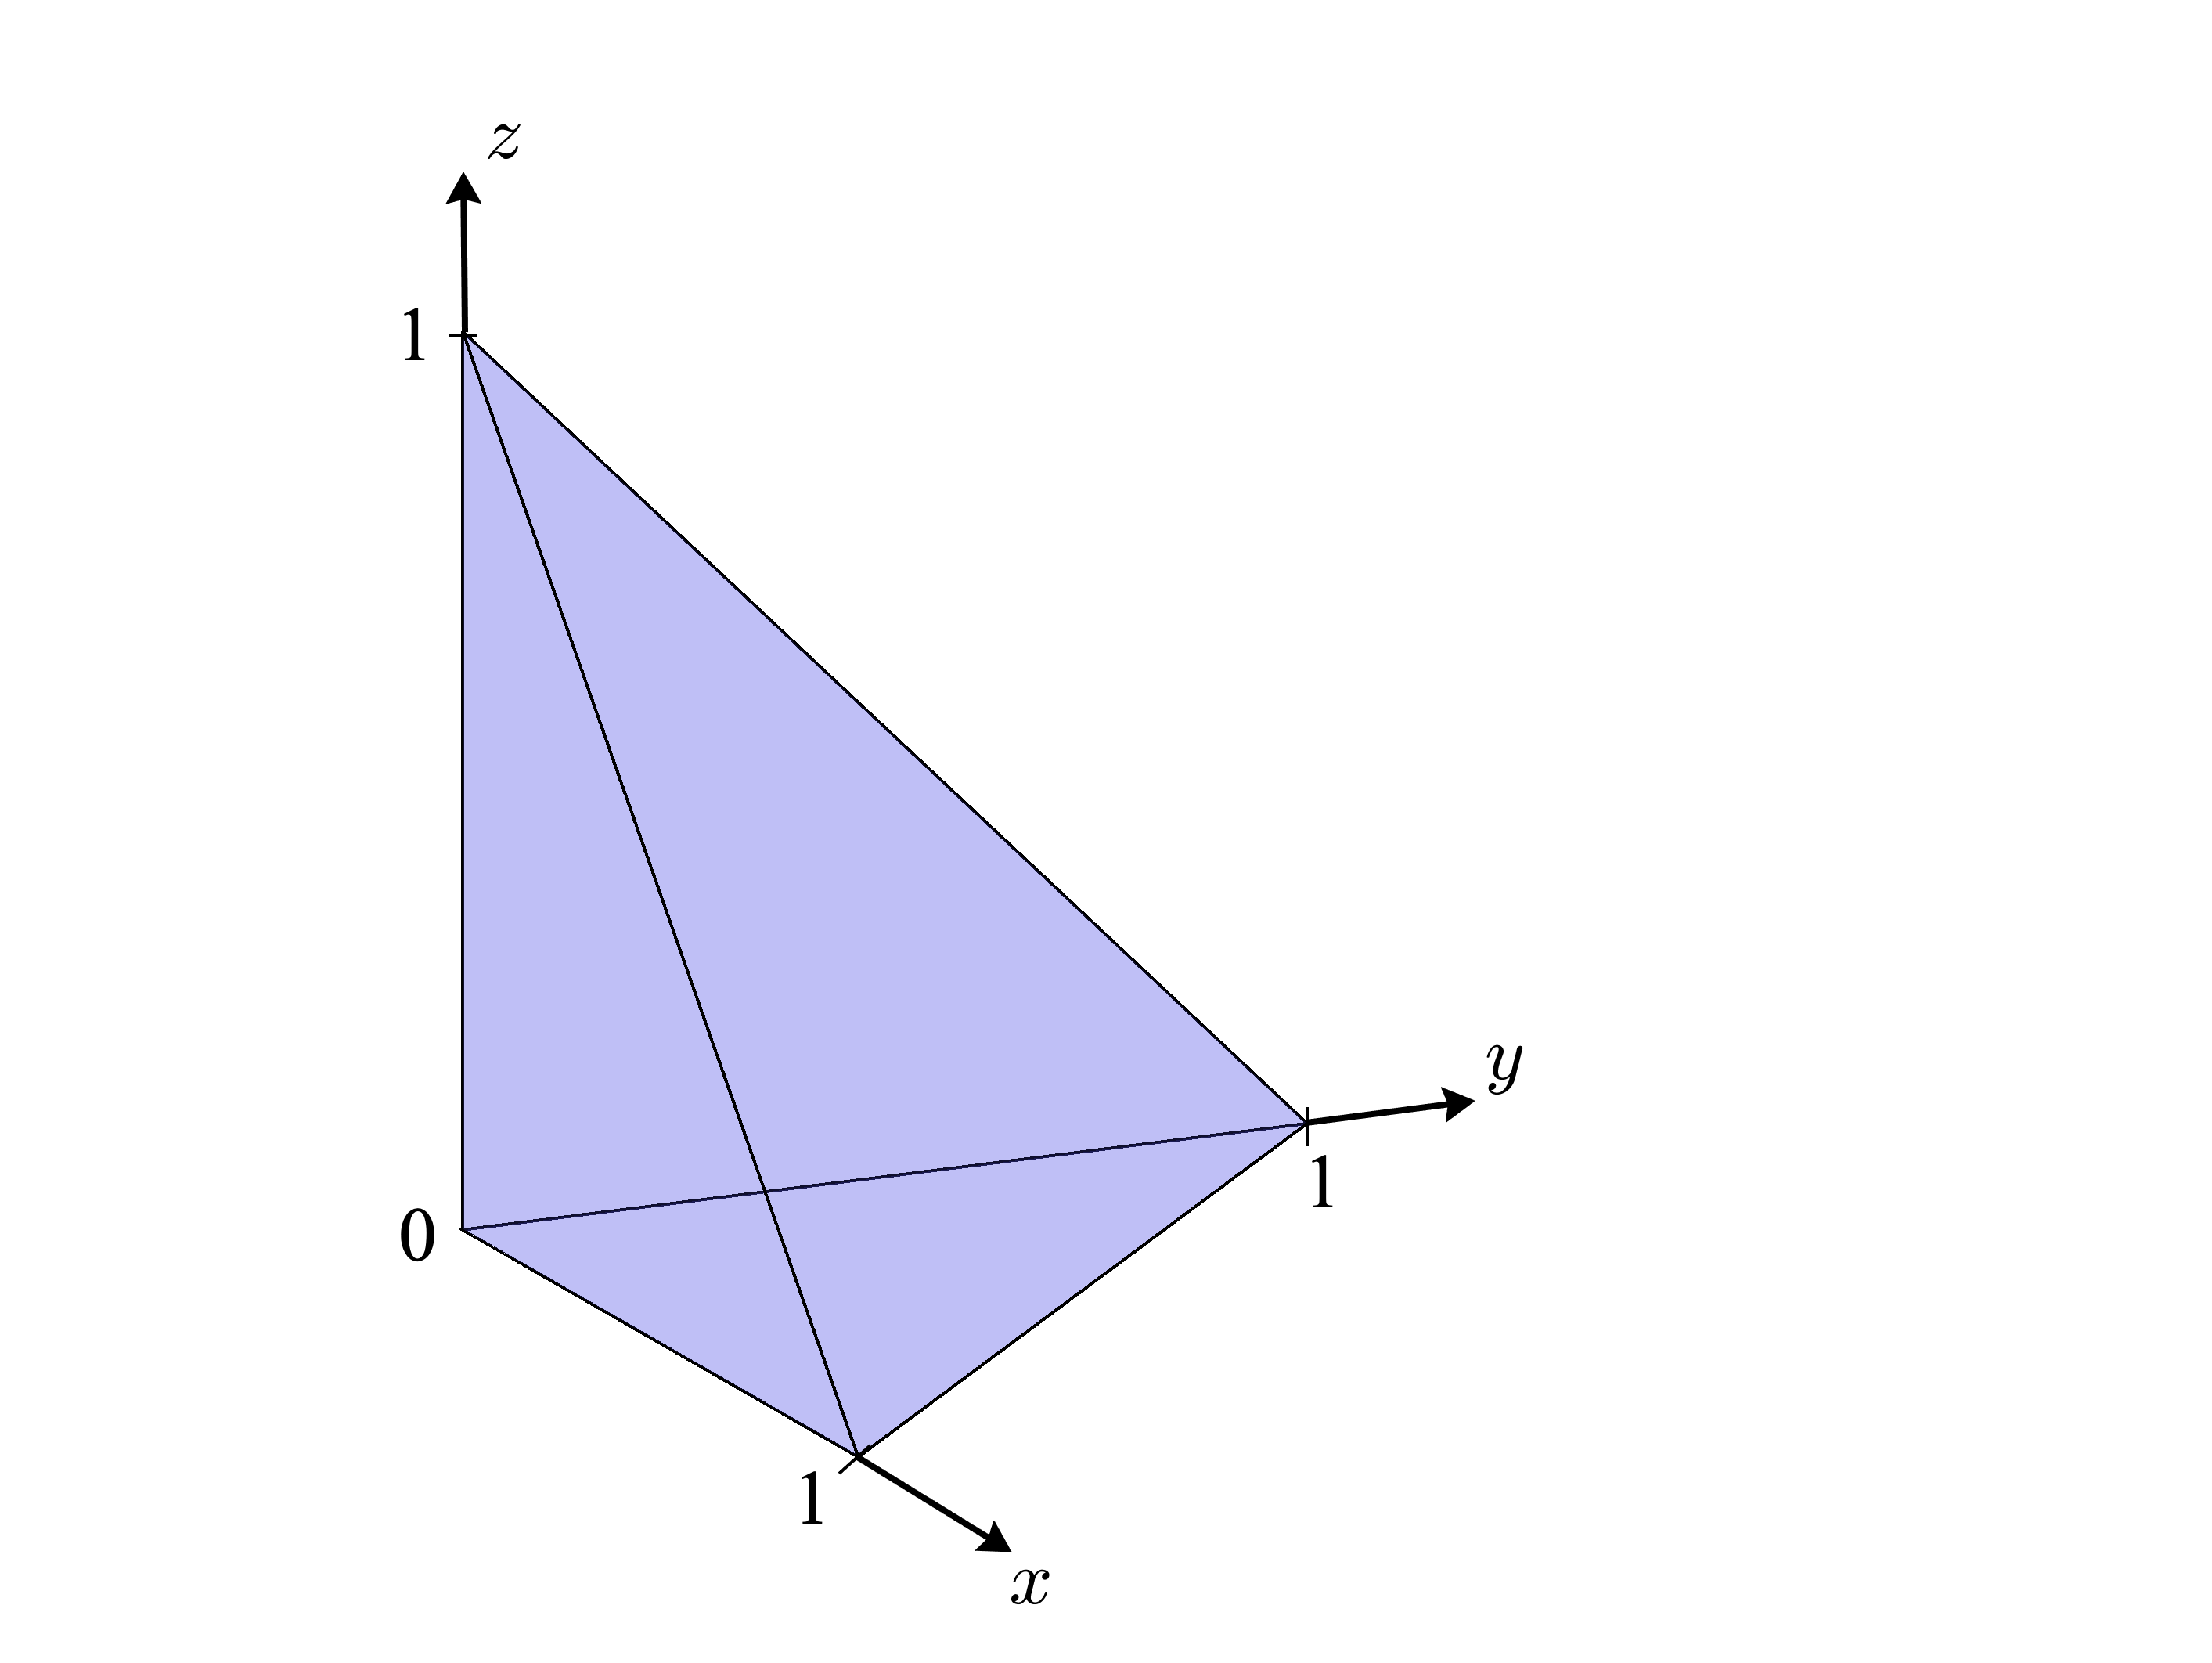
\includegraphics[width=8.7cm,height=6.9cm]{simplex}}
\caption{Subspace of interest for a 3-player generalized divide the dollar game without subsidies. Each point represents a set of bids where the $i$-th coordinate is the $i$-th player's bid. The triangle with vertices (1 0 0), (0 1 0), and (0 0 1) is a 2-simplex. Every point
on this surface has a bid total of \$1. All points on and beneath this surface represent coordinated bids. }
\label{fig1}
\end{figure}

Dan and I extended this by adding small \textcolor{purple}{\textit{subsidies}}. These subsidies allow the bid total to exceed $\$1$ and the players still get their bid as a payoff. However, the subsidies only apply if the bids are fair.  See Figure \ref{fig2}. The subsidy region is shown as a hemisphere extending from the 2-simplex surface. Notice the hemisphere is centered on the surface. (The center of the surface is the point where the bids are $\{1/3, 1/3, 1/3\}$.)

\begin{figure}[htb]
\centerline{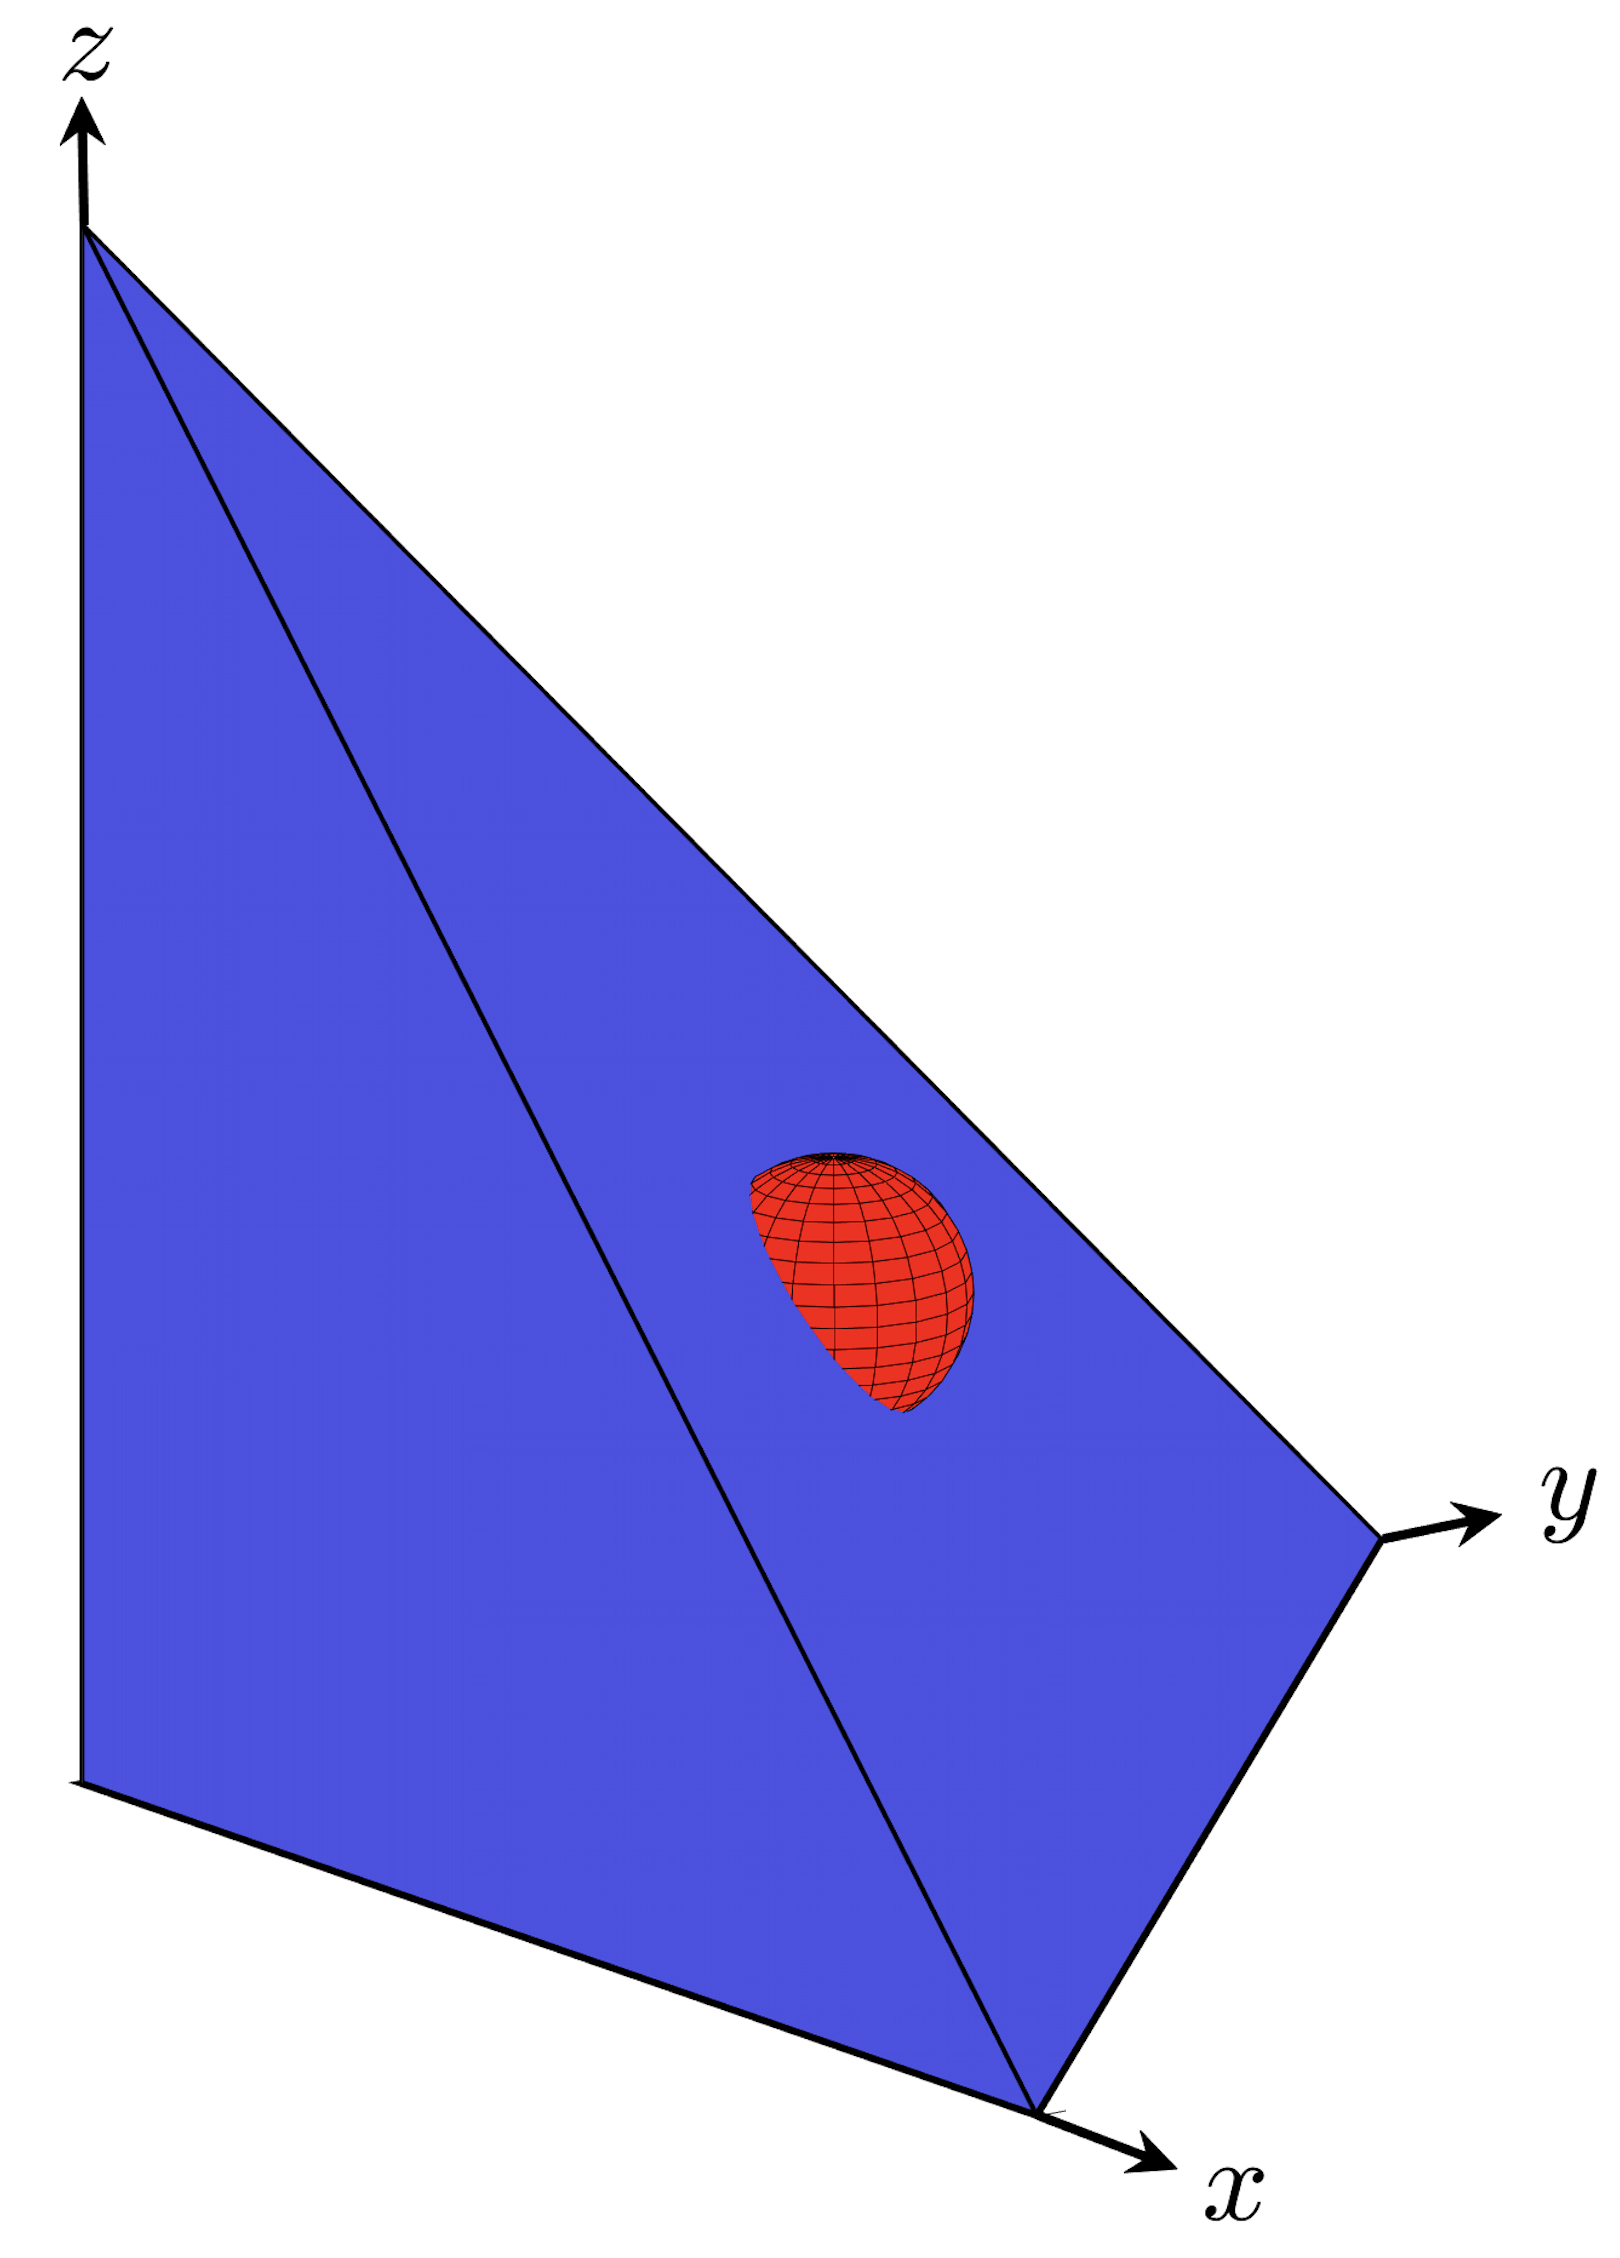
\includegraphics[width=5.7cm,height=7.9cm]{subsidize}}
\caption{Subspace of interest for a 3-player generalized divide the dollar game with subsidies. The hemisphere protruding from the 2-simplex face shows the subsidy region. }
\label{fig2}
\end{figure}

\subsection{NN player models}
Each player was modeled as a neural network as shown in Figure \ref{fig3}.  NNs are evaluated by participating in a series of 3-player tournaments. Let $n$ be the current time step. Referring to Figure \ref{fig3}, inputs $O_1$ and $O_2$ represent bids made by the two opponents in the two previous time steps $n-1$ and $n-2$. The input $C=\{0, 0.5\}$ denotes
whether the respective pair of bids plus the bid by the evaluated NN resulted in a coordinated bid (0.5 if coordinated bid, 0 if not).  For example, the 3-tuple $\{O_1^{n-1}, O_2^{n-1}, C^{n-1}\}=\{0.22, 0.63, 0\}$ indicates in the previous time step the two opponents bid 0.22 and 0.63 and the sum of the three bids was outside the coordinated bid subspace.

A CMA-ES algorithm evolved the weights and fitness was determined by 15-round tournaments amongst $k=3$ players---i.e., each player in the population competed in a tournament with all other player pairs and the outcomes were aggregated and then averaged over all such tournaments. High fitness was awarded if the bids were coordinated and fair. This was successful and a set of 3 high performing NN players were taken from the final population.
\begin{figure}[htb]
\centerline{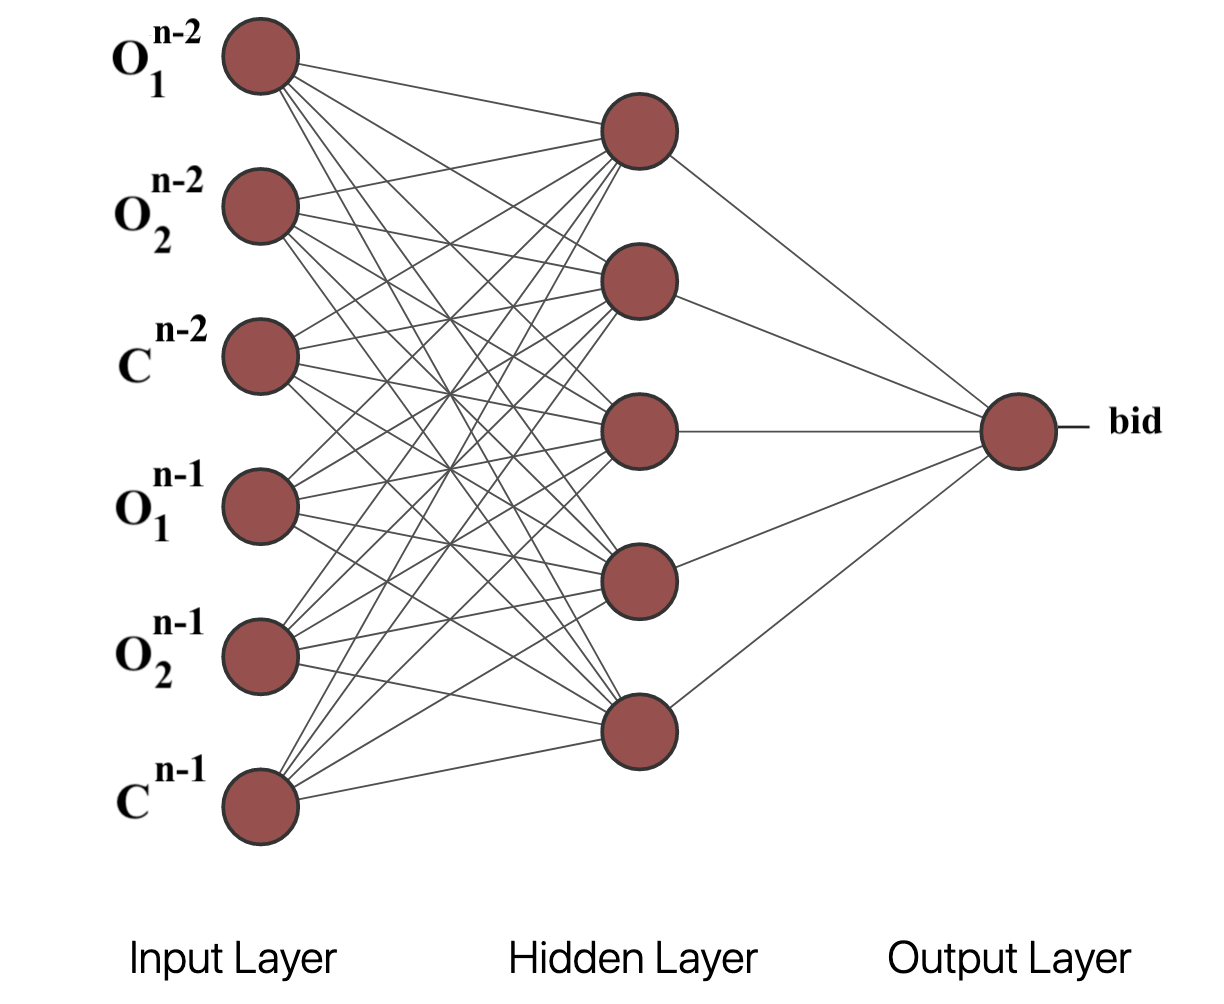
\includegraphics[width=9cm,height=7cm]{arch}}
\caption{The NN architecture. See text for explanation of inputs.}
\label{fig3}
\end{figure}

\section{The Canberra Work}

\subsection{Explainable AI (XAI)}

A machine learning (ML) model receives an $n$-dimensional input of features and outputs a prediction (see Figure \ref{fig3}). In classifier systems the model output is a value from a finite set; in regression systems the model output is a real-number.


XAI tries to explain or justify a given $p$ for a specific $x$ input. The problem is ML models are usually a black box so it is difficult---if not impossible---to explain how the model arrived at particular prediction. For example, the ML model could be a NN with 2 or 3 hidden layers. How do the synaptic weight values on the hidden layer nodes reflect which features were most important in generating $p$?


\begin{figure}[htb]
\centerline{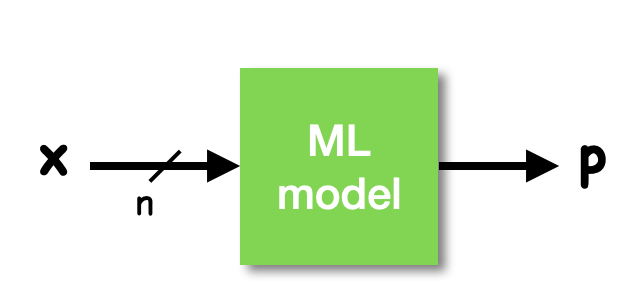
\includegraphics[width=6.7cm,height=3.2cm]{ML}}
\caption{A machine learning (ML) model. The input $x$ is an $n$-dimensional feature vector and the output $p$ is the prediction. }
\label{fig4}
\end{figure}

So if the ML model is a NN, we can't really explain how a particular prediction was determined. But what if we had a simpler ML model like a linear regression model that approximated the original model? Then we could explain a particular prediction because the coefficients in the regression equation indicate how much importance is attributed to each feature.

This leads to the notion of a \textcolor{red}{\textit{explainer model}}. The nice thing about explainer models is they \textit{can} be analyzed to see which features are most important in generating a prediction. Examples of explainer models include linear regressors, logistic regressors and random forests. Explainer models are trained using feature vectors from a database. The same training set used to design say a NN ML model would be used to train the explainer model.  A properly trained explainer model would output a prediction $p^{\prime} \approx p$ for the same input $x$ (see Figure 5). 

\begin{figure}[htb]
\centerline{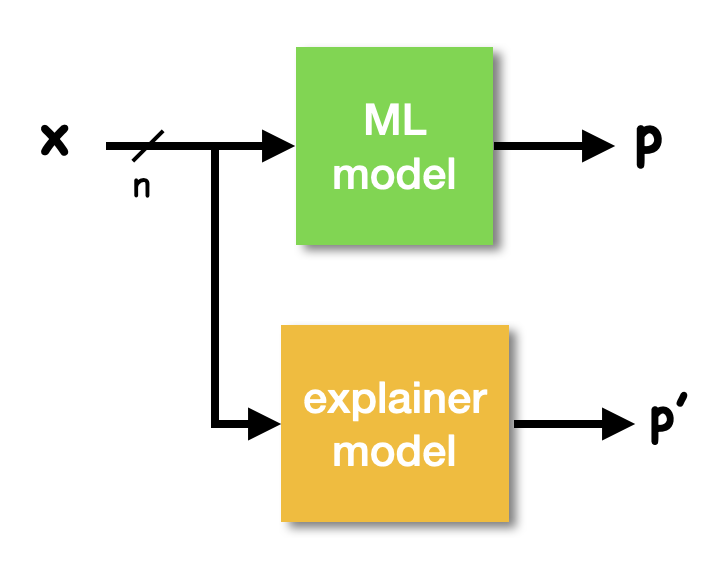
\includegraphics[width=6.7cm,height=4.9cm]{explainer}}
\caption{A properly trained explainer model emulates a ML model such as a NN.}
\label{fig5}
\end{figure}


\subsection{Shapley Values and SHAP}

Lloyd Shapley developed the Shapley values back in the 1950s. He later won the Nobel prize in economics for this work. The Shapley values were developed in a game theory context. 

Suppose $N$ players cooperate to achieve some outcome. The Shapley values indicate fair individual player payoffs based on their contribution to the outcome. SHAP\footnotemark was developed about 7 or 8 years ago. It extended Shapley values to the ML domain. Now ``players'' are ``features'' input to a ML model. SHAP estimates the Shapley values thereby indicated which features contributed the most to a given prediction.

\footnotetext{SHAP is the acronym for \textbf{SH}apley \textbf{A}dditive ex\textbf{P}lanations.}

Fortunately there are available a rich set of open-sourced library functions in python that compute SHAP values. I have this up and running.


\subsection{Objective}


In this work the ``features'' are the $O_i$ and $C$ inputs shown in Figure \ref{fig3}. The output prediction is the bid total so we are dealing with a regression ML model. A block diagram of the ML model of interest here is shown in Figure \ref{fig6}.

\begin{figure}[htb]
\centerline{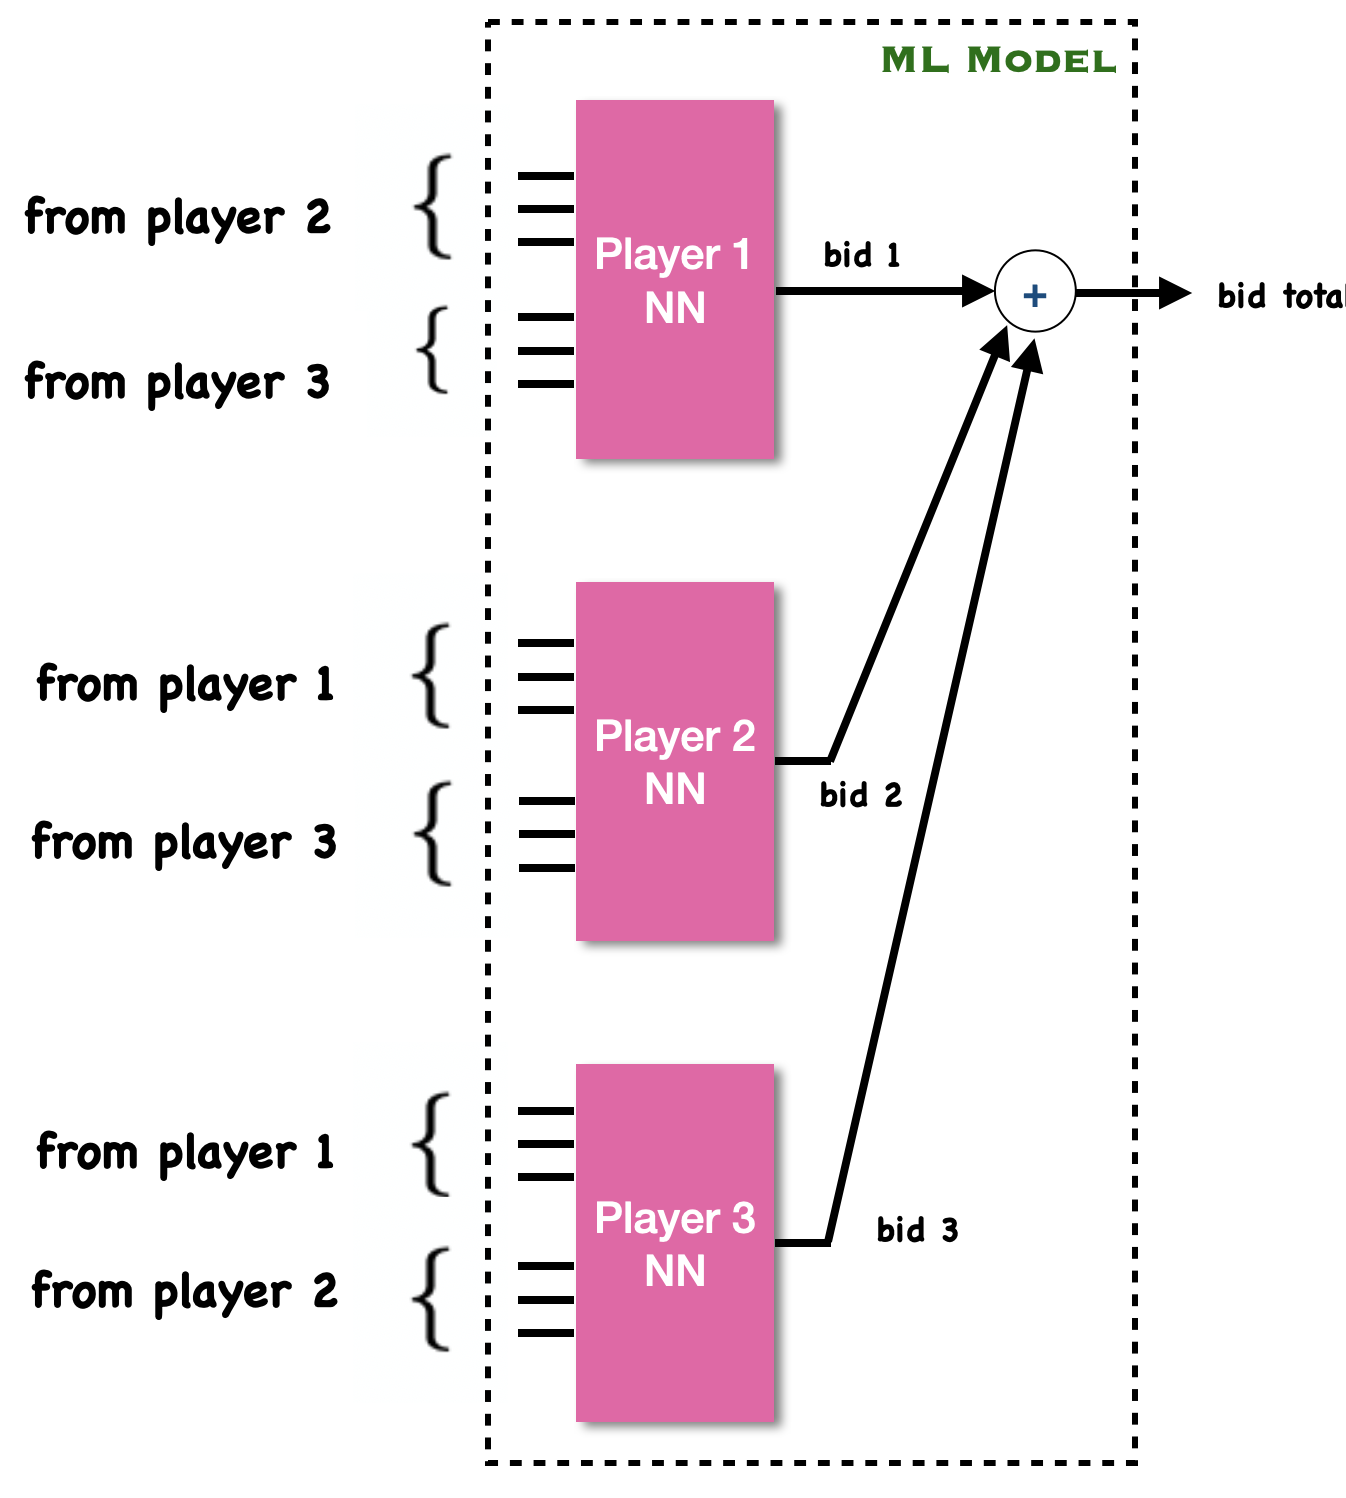
\includegraphics[width=7.7cm,height=7.9cm]{amy}}
\caption{The ML model. Each set of three inputs corresponds to the $O_1^{m}, O_2^{m}$ and $C^m$ NN inputs as shown in Figure \ref{fig3}.}
\label{fig6}
\end{figure}

The objective is to design an explainer model and then use SHAP to determine which features have the most affect on a prediction. Since the explainer model behaves like the original model, the features that most affect the explainer model predictions will be the same features most important to the original model predictions.

I am using a random forest as an explainer model.


\section{My Problem}

This is where I need some advice. 
\begin{table}[htb]
\begin{center}
\begin{tabular}{@{}clllc@{}}
\toprule
\multicolumn{1}{l}{\begin{tabular}[c]{@{}l@{}}vector \\ number\end{tabular}} & $f_1$ & $\cdots$ & $f_n$ & \multicolumn{1}{l}{prediction} \\ \midrule
1                                                                            & 0.22  &          & 0.93  & 0.49                           \\
2                                                                            & 0.17  &          & 0.69  & 0.71                           \\
\multicolumn{1}{c}{$\vdots$}                                                 &       &          &       & \multicolumn{1}{l}{}           \\
$N$                                                                          & 0.07  &          & 0.71  & 0.63                          
\end{tabular}
\caption{a sample training database}
\label{t1}
\end{center}
\end{table}

Suppose we have a database like that shown in Table \ref{t1}. There are $N$ feature vectors where $f_j$ is the $j$-th feature. In principle this database would be used to design both the ML model and the explainer model. But therein lies my problem: \textit{I don't have such a training database!!}

The NN players were not trained using a database. The synaptic weights were evolved using a CMA-ES algorithm. Fitness was determined by playing against pairs of other players in a series of tournaments. I need a database to train the explainer model.

In the MATLAB code I have a routine that will apply an 18-dimensional feature vector to the 3 NNs and get the bid total output (which is the prediction). I used the following method of generating a database: add noise to a feature vector and then run it through the NN model to get a prediction.  This process was repeated to create $N$ vectors. For the $O_1^m$ and $O_2^m$ inputs I took a nominal value of 0.3 and added to it a normally distributed random variable $\mathcal{N}(0,\sigma)$. 

The problem is what do I do for the $C^m$ inputs to randomize them? 
I tried picking 0 or 0.5 with equal probability, but when I did the SHAP analysis it said two (but not all) of the $C$ inputs had the most affect on the prediction. I guess that makes sense because it says the most important feature is whether or not the bid from the evaluated NN resulted in a coordinated bid total in the previous two rounds. But if that's true, why weren't \textit{all} of the $C^m$ inputs the most important features? Why only two and not all six?

So here are my questions:
\begin{enumerate}
\item Is there a better way to randomize the inputs $O^m$ inputs to create the training database?
\item What is the best way to randomize the $C$ inputs?
\item What should $N$ (the database size) be? 
\item Is there a better way to create a training database than what I described?
\end{enumerate}

Regarding the last two notes. Although $N=400$, it was actually split into a training set (320 vectors) and a test set (80 vectors). The SHAP library routines used the training vectors and the test vectors to create the random forest explainer model.

  Any comments would be most welcome. If necessary, we can set up a zoom call to talk. Let me know.

\end{document}  